\documentclass{beamer}

\usepackage[utf8]{inputenc}
\usepackage{amsmath}
\usepackage{amsfonts}
\usepackage{amssymb}
\usepackage{amsthm}
\usepackage[ukrainian,russian]{babel}
\usepackage{ulem}

\usepackage{fontenc}
\usepackage{graphicx}
% \usepackage{default}
\usetheme{Warsaw}
% \author{Ширай Андрей}
 \institute{Кафедра медичної інформатики та комп'ютерних технологій навчання ,\\
    Національний медичний університет імені О.О.Богомольця}
\title{Биостатистика}
\begin{document}
\frame{\titlepage}

\frame{
  \frametitle{Выучи теорию вероятностей за 15мин для чайников}

  \begin{itemize}
  \item \Large Вероятность, Случайная величина
    

   \item Матожидание и Дисперсия
     
   
  \item Плотность вероятности, Вероятностные распределения
    

  \item Центральная предельная теорема
    
  \end{itemize}
}

 
\frame{
\frametitle{Вероятность, рабоче-крестьянское определение...}
\Large
Вероятность -- это \textit{мера} возможности появления какого-либо случайного события.

}

\frame{
\frametitle{Вероятность, рабоче-крестьянское определение...}
\Large
Вероятность -- это \textit{мера} возможности появления какого-либо случайного события.
\resizebox{.6\hsize}{!}{$P(A)=\frac{\left | A \right |}{\left | \Omega  \right |}$} 
}

\frame{
\frametitle{Вероятность, рабоче-крестьянское определение...}
\Large
Вероятность -- это \textit{мера} возможности появления какого-либо случайного события.
\resizebox{.6\hsize}{!}{$P(A)=\frac{\left | A \right |}{\left | \Omega  \right |}$} 
\begin{tabular}{ccc}
$\left | A \right |$ -- Количество реализаций события А \\
$\left | \Omega  \right | $ -- Общее количество всех возможных случаев
\end{tabular}
}

\frame{
  \frametitle{Вероятность}

\begin{tabular}{ccc}
\resizebox{.6\hsize}{!}{$P(A)=\frac{\left | A \right |}{\left | \Omega  \right |}$} &  \\ 
\\ 
\resizebox{.4\hsize}{!}{$ \Omega=\left \{ \text{орел, решка } \right \}$} & \resizebox{.4\hsize}{!}{$ \Omega=\left \{ 1, 2, 3, 4, 5, 6 \right \}$}\\
\resizebox{.4\hsize}{!}{$A=\text{орел}$} & \resizebox{.4\hsize}{!}{$A=\left \{ 5,6\right \}$}  \\ 
\resizebox{.4\hsize}{!}{$P(A)=\frac{\left | A \right |}{\left | \Omega  \right |} = \frac{1}{2}$ } & \resizebox{.4\hsize}{!}{$P(A)=\frac{\left | A \right |}{\left | \Omega  \right |} = \frac{2}{6}= \frac{1}{3}$ }
\end{tabular}
}

\frame{
  \frametitle{Случайная величина}
 \begin{itemize}
\item \textbf{Случайная величина} (почти) любая\footnote{измеримая} вещественная функция от случайного события: 


\resizebox{.2\hsize}{!}{$\xi : \Omega \to \mathbb{R}$}

\item Пример:
\[
Y(\omega) = \begin{cases}
          1, & \text{if} \ \ \omega = \text{heads} ,\\
          0, & \text{if} \ \ \omega = \text{tails} .
        \end{cases}
\]

\end{itemize}
}


\frame{
  \frametitle{Функция и Плотность распределения}
 \begin{itemize}
\item \textbf{Функция распределения}: $F_{\xi}(x)=P\{\xi < x\}$

\item \textbf{Плотность распределения}: Если существует функция $p(x)$, что: $F_{\xi}(y)=\int_{-\infty}^yp(x)dx$, то говорят что случайная величина имеет плотность $p(x)$

\item $P(a<\xi<b)=\int_a^bp(x)dx$
\end{itemize}
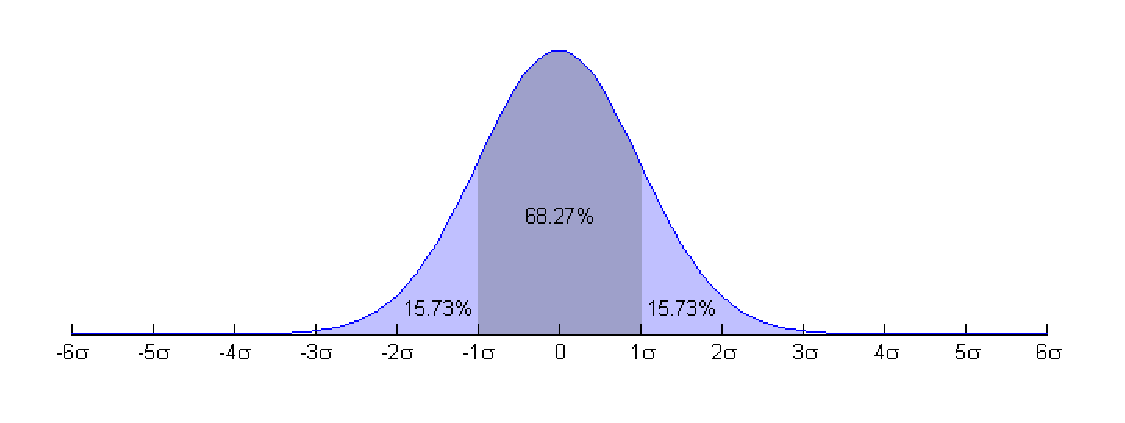
\includegraphics[scale=0.5]{den} 
}


\frame{
  \frametitle{Матожидание}
 \begin{itemize}
\item \textbf{Математическое ожидание} случайной величины -- это средневзвешенное среднее. 

\item Дискретный случай: $\operatorname{M}[\xi] = \sum_{i} x_i\, p_i$

\item Непрерывный случай: $\operatorname{M}[\xi] = \int_{-\infty}^\infty x p(x)\, \operatorname{d}x$

\item Пример:

 $\xi$ -- число, выпавшее после подкидывание кубика d6. Возможные значения $\xi$: 1, 2, 3, 4, 5, 6, все с вероятностью $\frac{1}{6}$. Матожидание $X$:
\[
    \operatorname{M}[\xi] = 1\cdot\frac16 + 2\cdot\frac16 + 3\cdot\frac16 + 4\cdot\frac16 + 5\cdot\frac16 + 6\cdot\frac16 = 3.5.
\]
\end{itemize}
}

\frame{
  \frametitle{Свойства матожидания}
\begin{itemize}
 \item $M[c] = c, \forall c \equiv \text{const} $ 
\item $M[a\xi + b\mu]= aM[\xi] + bM[\mu]$
\end{itemize}


}
\frame{
  \frametitle{Дисперсия}
 \begin{itemize}
\item \textbf{Дисперсия} -- среднее значение квадрата отклонения случайной величины от ее среднего . 

\item Если $\xi$ имеет \textbf{матожидание} $\mu = M[\xi]$, то дисперсия $\xi$:
\[
        \operatorname{D}(\xi) = \operatorname{M}[(\xi - \mu)^2] 
% =  \operatorname{M}[\xi^2] - (\operatorname{M}[\xi])^2
\]
\item "Физический смысл": дисперсия -- это степень разброса значений
\item Для дискретной случайной величины: $\operatorname{Var}(X) = \sum_{i=1}^n p_i\cdot(x_i - \mu)^2 $, где $\mu = \sum_{i=1}^n p_i\cdot x_i$
\item $\xi$ -- число, выпавшее после подкидывание кубика d6. Дисперсия $X$:
$
\sum_{i=1}^6 \tfrac{1}{6}(i - 3.5)^2 = \tfrac{1}{6}\sum_{i=1}^6 (i - 3.5)^2  = \tfrac{1}{6}\left((-2.5)^2{+}(-1.5)^2{+}(-0.5)^2{+}0.5^2{+}1.5^2{+}2.5^2\right) = \tfrac{1}{6} \cdot 17.50 = \tfrac{35}{12} \approx 2.92
$
% \[\sum_{i=1}^6 \tfrac{1}{6}(i - 3.5)^2 = \tfrac{1}{6}\sum_{i=1}^6 (i - 3.5)^2  = \tfrac{1}{6}\left((-2.5)^2{+}(-1.5)^2{+}(-0.5)^2{+}0.5^2{+}1.5^2{+}2.5^2\right) \\
%  = \tfrac{1}{6} \cdot 17.50 = \tfrac{35}{12} \approx 2.92 \]
\end{itemize}
}

\frame{
  \frametitle{Свойства дисперсии}
 \begin{itemize}
  \item  $ \operatorname{D}(\xi) = \operatorname{M}[(\xi - \mu)^2] = \operatorname{M}[\xi^2] - (\operatorname{M}[\xi])^2$
\item $D[c\xi]=c^2D[\xi]$
\item $D[\xi]\geq 0$, $D[\xi] = 0 \Leftrightarrow \xi = 0$
\item $D[\xi+c]= D[\xi]$
 \end{itemize}

}

\frame{
  \frametitle{Равномерное распределение}

\begin{itemize}
\item Плотность: $\begin{cases}
                  \frac{1}{b - a} & \text{если } x \in [a,b]  \\
                  0               & \text{иначе}
                \end{cases}$
\item $\operatorname{M}[\xi]=\tfrac{1}{2}(a+b)$, $\operatorname{D}[\xi]=\tfrac{1}{12}(b-a)^2$
\end{itemize}
\includegraphics[scale=0.15]{uni} 
}

\frame{
  \frametitle{Распределение Пуассона}
\begin{itemize}
\item  Плотность: $p(X=k)=\frac{\lambda^k e^{-\lambda}}{k!}\!$
\item $\operatorname{M}[X]=\lambda$, $\operatorname{D}[X]=\lambda$
\end{itemize}
\includegraphics[scale=0.5]{pois} 
}

\frame{
  \frametitle{Нормальное распределение}
\begin{itemize}
\item Плотность: $\tfrac{1}{\sqrt{2\pi\sigma^2}}\,e^{ -\frac{(x-\mu)^2}{2\sigma^2} }$
\item $\operatorname{M}[\xi]=\mu$, $\operatorname{D}[\xi]=\sigma$

\end{itemize}
\includegraphics[scale=0.25]{norm} 

}

 \frame{
   \frametitle{Центральная предельная теорема}
 
 Пускай $\xi_1,\xi_2,\dots \xi_n$ --независимые одинаковораспределенные случайные величины. Тогда:
\[
 \frac{S_n -n\mu }{\sqrt{n}\sigma} \xrightarrow{d} N(0,1), \mu = \operatorname{M}\xi_i , \sigma = \operatorname{D}\xi_i, S_n = \sum_n\xi_i
\]



 }

% % % % % % % % % % % % % % 
%  Перерыв
% % % % % % % % % % % % % % 

% \frame{
% \frametitle{Break}
% \Huge Let's have a \textbf{break}!
% 
% 
% }

%%%%%%%%%%%%%%%%%%%%%%%%%%%%%%%%%%%%%%%%%%%%%%
 \frame{
   \frametitle{Биостатистика}
 
   \begin{itemize}
   \item \Large \sout{Статистика и биология}
     
 
   \item Эксперимент и наблюдение
     
   
    \item Основные статистические характеристики выборки
 
   \item Корреляция и Регрессия
   \item  \sout{Тестирование гипотез}\footnote{Рассмотрим на следующей практике}  
     
   \end{itemize}
 }


\frame{
  \frametitle{Почему статистика так важна?}
\Huge Ложь, наглая ложь и \textbf{статистика}
}


\frame{
  \frametitle{Выборка и Генеральная совокупность}
\begin{itemize}
\item \textbf{Выборка} -- наблюдения одной и той же случайной величины, при повторных случайных экспериментах.
\item Проще говоря выборка -- это результаты эксперимента.
\item \textbf{Вариационный ряд} - значения выборки, упорядоченные по неубыванию.
\end{itemize}
}

\frame{
  \frametitle{Среднее, Мода, Медиана. Дисперсия, Отклонение }
\begin{itemize}
\item \textbf{Выборочное матожидание}: $\bar{x}=\frac{1}{N}\sum_{k=1}^{N}x_k$
\item \textbf{Мода} -- значение, которое встречается в выборке чаще всего
\item \textbf{Медиана}  -- значение, которое дели вариационный ряд на 2 половины
\item \textbf{Выборочная дисперсия}: $\sigma_N^2 =  \frac{1}{N-1}\sum_{i=1}^n \left(x_i - \overline{x} \right)^ 2$
\item \textbf{Среднеквадратичное(Стандартное) отклонение}: $\sigma_N = \sqrt{\frac{1}{N-1} \sum_{i=1}^N (x_i - \overline{x})^2}$
\end{itemize}
}



\frame{
  \frametitle{Гистограмма}
\textbf{Эмпирическая функция распределения}: $F_n(x)=\frac{1}{n}\sum_{i=0}^nI_{x_i \leq x}$

\textbf{Гистограмма}: 
\[
p_{n}(x)= \sum_{k=1}^{N}\frac{1}{\left | \Delta_k \right |}v_kI_{\Delta_k}(x), v_k = \frac{1}{n}\sum_{n}^{j=1}I_{\Delta_k}(X_j)
\]
\includegraphics[scale=0.2]{hist} 

}

\frame{
  \frametitle{Ошибка репрезентативности}
\begin{itemize}
\item \textbf{Ошибка репрезентативности} -- ошибка, которая вызвана тем, что мы работаем с выборкой, а не всей генеральной совокупностью: 

\[
m = \frac{\sigma }{\sqrt{N}}
\]
 $\sigma$ -- среднеквадратичное отклонение, $N$ -- размер выборки
\end{itemize}
}

\frame{
  \frametitle{Корреляция}
\begin{itemize}
\item  \textbf{Корреляция} -- степень зависимости между двумя наблюдаемыми случайными величинами.
\item  Степень \textit{линейной} зависимости показывает \textbf{коэфициент корреляции Пирсона}: 
\[
 \mathbb{R}_{X,Y} = \frac{\mathrm{cov}(X,Y)}{\sigma_X \cdot \sigma_Y} = \frac{1}{n} \frac{\sum\limits_{i=1}^n (x_i-\bar{x})(y_i-\bar{y})}{\sigma_X \cdot \sigma_Y}
\]
%  

\begin{center}
    \begin{tabular}{ | p{3cm}  | p{3cm}  |}
\hline
Корреляция & $ \left | \mathbb{R}_{X,Y} \right |$ \\ \hline
Отсутствует & 0.0 to 0.09 \\ \hline
Слабая & 0.1 to 0.3 \\ \hline
Умеренная & 0.3 to 0.5 \\ \hline
Сильная & 0.5 to 1.0 \\ \hline
 \end{tabular}
\end{center}
\end{itemize}
}
\frame{
  \frametitle{Корреляция -- диаграммы рассеивания}
\includegraphics[scale=0.35]{cor}
}
% \frame{
%   \frametitle{Correlation - example}
% 
% }
\frame{
  \frametitle{Модель регрессии}
\begin{itemize}
\item У нас есть две парные выборки X и Y
\item Необходимо построить кривую, которая отображает зависимость Y(X)
\item Вид зависимости задается эмпирически(те. угадывается)
\item Для построения кривой чаще всего пользуются -- \textbf{методом наименьших квадратов}:
\item Из всех возможных кривых мы выбираем такую, что сумма квадратов расстояний до не от всех точек минимальна.
\end{itemize}

}
 \frame{
   \frametitle{Линейная оценка МНК в модели регрессии}
\begin{itemize}
 \item $y = kx +b$
\item Тут $<x>$ -- среднее величины х
\item $k=\frac{<x^2><y> - <x><xy>}{<x^2>-<x>^2}$
\item $b=\frac{<xy> - <x><y>}{<x^2>-<x>^2}$
\end{itemize}

 }
\frame{
  \frametitle{Модель регрессии}
\includegraphics[scale=0.5]{ls} 
}


% 
% \frame{
%   \frametitle{Нелинейные зависимости}
% }
% 
% \frame{
%   \frametitle{Нелинейные зависимости -- пример}
% }

\frame{
  \frametitle{Post hoc ergo propter hoc}
\includegraphics[scale=0.35]{pirates}
}
\frame{
  \frametitle{Post hoc ergo propter hoc}
\includegraphics[scale=0.7]{correlation}
}

% \frame{
%   \frametitle{Тестирование гипотез}
% \begin{itemize}
% \item A statistical hypothesis test is a method of making decisions using data
%  \item A result is called \textbf{statistically significant} if it is unlikely to have occurred by chance alone, according to a pre-determined threshold probability, the \textbf{significance level}.
% \item A result that was found to be statistically significant is also called a \textbf{positive result}; conversely, a result whose probability under the null hypothesis exceeds the significance level is called a negative result or a null result.
% \end{itemize}
% }
% 
% \frame{
%   \frametitle{Ошибки первого и второго рода}
% \begin{center}
%     \begin{tabular}{ | p{3cm}  | p{3cm}  | p{3cm}  |}
%     \hline
%      & Null Hypothesis ($H_{0}$) is true & Alternative Hypothesis ($H_{1}$) is true  \\ \hline
%      Fail to Reject Null Hypothesis & Right decision & Type II Error  \\ \hline
%      Reject Null Hypothesis & Type I Error &Right decision  \\ \hline
%     \end{tabular}
% \end{center}
% }
% 
% \frame{
%   \frametitle{Тестирование гипотез}
% \begin{itemize}
% \item We start with a research hypothesis of which the truth is unknown.
% \item The first step is to state the relevant null and alternative hypotheses. This is important as mis-stating the hypotheses will muddy the rest of the process. 
% \item The second step is to consider the statistical assumptions being made about the sample in doing the test; for example, assumptions about the statistical independence or about the form of the distributions of the observations.
% \item Decide which test is appropriate, and stating the relevant test statistic.
% \item Derive the distribution of the test statistic under the null hypothesis from the assumptions. 
% \item Compute from the observations the observed value tobs of the test statistic T.
% \item Decide to either fail to reject the null hypothesis or reject it in favor of the alternative. 
% \end{itemize}
% }
%  \frame{
%    \frametitle{Критерий Пирсона $\chi^2$ }
%  
%  }
%  \frame{
%    \frametitle{Критерий Пирсона  $\chi^2$ -- алгоритм}
%  
%  }
%  \frame{
%    \frametitle{Критерий Пирсона $\chi^2$ -- пример}
%  
%  }
% \frame{
% \frametitle{Какой критерий выбрать?}
% 
% 
% }

\frame{
\frametitle{Dixi}

\begin{center}
\Huge Dixi\end{center}
}
\end{document}
